
\chapter{The experiment}

\section{Large Hadron Collider}

The Large Hadron Collider (LHC) has a radius of approximately 27 kilometers. As of this writing, it is the largest machine ever constructed. The initial purpose of the LHC was to discover the Higgs boson, but it is capable of investigating a variety of other physics phenomena, such as dark matter, extra-dimensions, and heavy-ion physics.

The beams are accelerated along a circular path using radio frequency cavities, gaining energy with each revolution. LHC is a hadron collider, meaning it is designed to collide particles made of quarks and gluons. The proton-proton, proton-Pb, and Pb-Pb collision energies are the largest ever probed experimentally. The LHC is a circular collider.

Heavy-ion collisions at LHC produce strongly interacting nuclear matter. The temperature and density of this matter is comparable to the state of the universe only a few milliseconds after the Big Bang.

\subsection{ATLAS}

"ATLAS" stands for "A Toroidal LHC ApparatuS". ATLAS was designed as a general purpose detector for LHC physics. Three toroidal superconducting magnets provide the field for particle identification, in contrast to the titular compact solenoid magnet of CMS. The looser design constraints of the ATLAS magnets allow for a more efficient, stand-alone measurement of muon momentum. 

\subsection{ALICE}

"ALICE" stands for "A Large Ion Collider Experiment". ALICE, unlike ATLAS and CMS, is not a general purpose detector. ALICE was designed to study a specific phenomena: the quark-gluon plasma posited to exist during ultra-relativistic heavy-ion collisions. The primary design consideration was the correct identification of particle species at high multiplicities. ALICE retains excellent PID at approximately $dN / d\eta = 4000$, and this over a particle momentum range up to 100 GeV. PID is accomplished through a combination of time-of-flight chambers, muon filters, and the analysis of specific ionization energy. 

\subsection{LHCb}

"LHCb" stands for "Large Hadron Collider beauty", reflecting the LHCb's purpose: b-quark ("beauty") studies. In this respect it is similar to ALICE, LHC's other specialized experiment. By examining CP violation in heavy-quark hadrons, LHCb hopes to elucidate the asymmetry of matter and antimatter. LHCb is asymmetric in the z-axis: b-hadron pairs tend to scatter in the same forward rapidity, so the experiment only covers $1.9<\eta<4.9$. A large dipole magnet projects an field in the vertical plane of LHC. Small asymmetries in the transverse scattering of the b-hadron system are used to test for CP violation. 

\subsection{TOTEM}

"TOTEM" is a sub-experiment located at CMS. TOTEM uses Roman Pots (RPS), placed far forward of CMS, to measure the total proton+proton interaction cross-section. The RPS have high acceptance for the flux very close to the beam. There are two sets of RPS, one on each side of CMS, located approximately 400 meters down the z-axis from the interaction point. The differential cross-section, of proton-proton scattering, grows exponentially with the $|t|$ at low values of $|t|$. More precise measurements of this differential cross section can help distinguish between competing models of proton structure. Furthermore, the total interaction cross-section is an important benchmark for analyzing cosmic ray showers, and can be used to independently calibrate the beam luminosity measured at other LHC experiments. Diffractive studies at TOTEM complement those at CMS.

\section{Compact Muon Solenoid}

The Compact Muon Solenoid (CMS) is a general-purpose particle detector located at Point-5 of the LHC. CMS was designed to precisely measure the momentum of muons. The titular superconducting solenoid magnet was designed to generate a 4 Tesla field, but operates at 3.8 T to increase longevity. This field is homogeneous and parallel to the beam line close to the interaction point. The momentum of a muon is measured from how it deflects when moving through the magnetic field. Altogether, CMS weighs approximately 12,500 metric tons, with a diameter of 14.6 m and a length of 21.6 meters. Fig.\ref{fig:cmsCutOut} displays the detector's various sub-systems. 

\begin{figure}[h!]
\begin{centering}
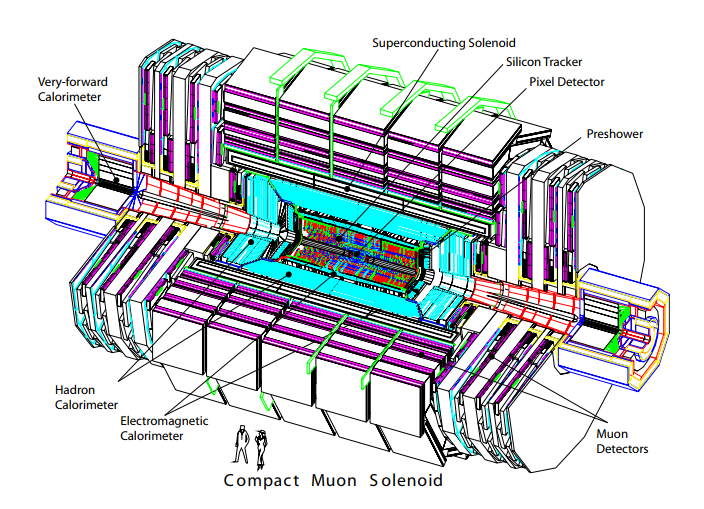
\includegraphics[width=4in]{Chapter3/importfigs/fromCMS_DesignPaper_perspective.png}
\par\end{centering}
\caption{CMS Detector \label{fig:cmsCutOut}}
\end{figure}

Within the solenoid volume are a silicon pixel and strip tracker, a lead tungsten crystal electromagnetic calorimeter (ECAL), and a brass and scintillator hadron calorimeter (HCAL), each composed of a barrel and two endcap sections. Fig.\ref{fig:cmsCutOutZY} radial layering of CMS component systems.  

\begin{figure}[h!]
\begin{centering}
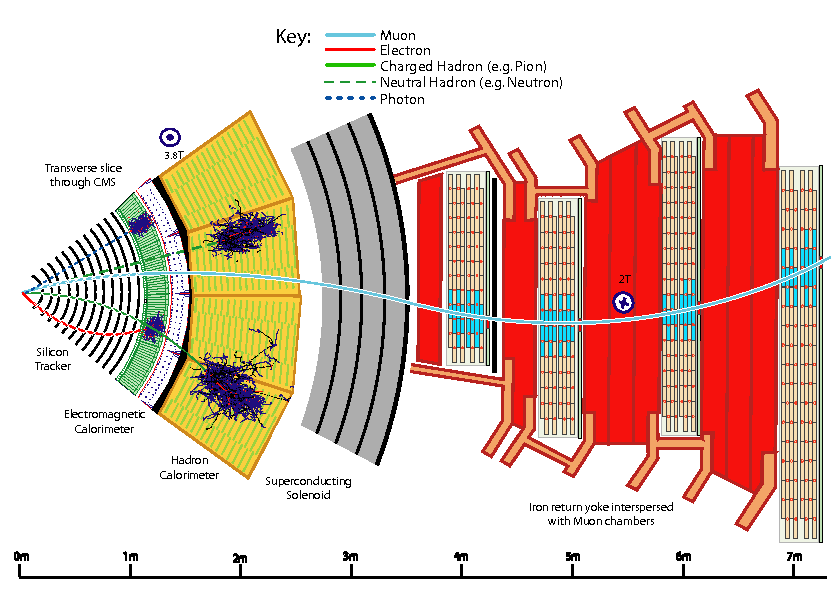
\includegraphics[width=5.5in]{Chapter3/importfigs/Figure_001.png}
\par\end{centering}
\caption{CMS radial cross-section \label{fig:cmsCutOutZY}}
\end{figure}

\subsection{Tracker}

The tracker measures the momentum of charged particles via their trajectory through a homogenous magnetic field. The tracker consists of two units, the pixel tracker and the strip tracker, both of which are made of silicon. Compared to large-volume gas detectors, which are less expensive, silicon detectors have a faster response time. The number of tracker layers is optimized for the highest penetration by charged particles while minimizing the occurence of multiple scattering. 

Multiple scattering reduces the efficiency and resolution of the tracker because of bremmstrahlung. When a charged lepton passes through an electric field, the changes in acceleration will change the energy of lepton. The lepton will release photons that will contaminate the signals read by the tracker. 

The high luminosities reached by LHC typically achieve some 20 to 30 collisions per bunch crossing, and increasing the number of hits in the tracker improves the pattern recognition of the particle flow algorithm. The particle flow algorithm is discussed in more detail later in this chapter. 

A charged particle causes an electrical signal when passing through a silicon pixel or silicon microstrip. CMS reconstructs these electrical signals, taken at specific points of position and time, into tracks. These tracks are accurate to 10 micrometers. The tracker is meant to have  a particle pass all the way through it, with only minimal effect particle's trajectory. 

The tracker system is designed for high granularity and fast readout, such that each trajectory can be associated with its corresponding bunch crossing. The tracker is resilient enough to withstand the high flux of particles accompanying every bunch crossing; at design luminosity of $10^34 cm^-2 s^-1$, some 1000 particles will traverse the tracker every 25 ns. However, the mass of the tracker is minimal enough to suppress multiple scattering, off its material, that would distort particle trajectories. These design constraints -- resistance and transparency -- are satisfied silicon. The tracker has approximately $200 m^2$ of silicon surface, making it the largest silicon detector ever constructed. The pseudorapidity coverage of the pixel and strip trackers is shown in fig.\ref{fig:trackerYZ}.

\begin{figure}[h!]
\begin{centering}
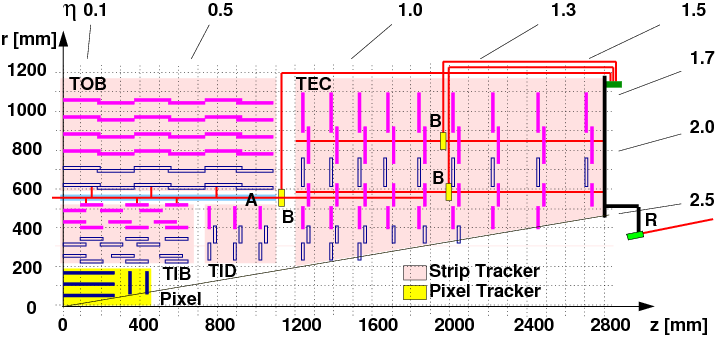
\includegraphics[width=4in]{Chapter3/importfigs/cms_cft_09_003_fig1.png}
\par\end{centering}
\caption{Pseudorapidity acceptance of tracker \label{fig:trackerYZ}}
\end{figure}

In addition to excellent track reconstruction, the tracker provides high precision vertex reconstruction. Vertex reconstruction is a key ingredient in several high-profile LHC studies -- Higgs, SUSY, extra-dimensions -- because of the use of vertices in distinguishing non-prompt decays of heavy-quarks. 

\subsubsection{Pixel tracker}

The first layer of the tracker is made of silicon pixel modules. This layer has a time resolution on the scale of 25 ns, meaning that it can take data for individual bunch crossings. Pixel technology is used because the high flux of particles, present at high beam luminosities, require high spatial resolution for proper pattern recognition. A major design constraint is that the pixel tracker had to be able to separate distinct tracks in high multiplicity environments. Tracks reconstructed by the pixels can be used to cross-check the results from the other parts of the tracker. 

Every silicon-pixel has a corresponding readout chip. The readout chips are soldered through the bump-bonding method. The readout chip amplifies signals from the pixel. The pixel tracker is precise enough to distinguish the vertices of tracks originating from short-lived particles, such as bottomonia. The innermost elements of the pixel tracker come within 4.4 cms of the CMS interaction point. The pixel tracker covers a pseudorapidity range of $|\eta|<2.5$ with some $66 \times 10^6$ separate pixels.

\subsubsection{Strip tracker}

Outside the pixel tracker are the layers of the strip tracker. They function similar to the components of the pixel tracker, except the strip tracker consists of thin silicon plates. The strip tracker itself can be broken down into four components: the inner barrel layer, the inner endcaps, the outer barrel layer, and the outer endcaps. In total, these layers contain some $9.3 \times 10^6$ strips. 

\subsection{Electromagnetic calorimeter}

The Electromagnetic Calorimeter (ECAL) is the dedicated CMS calorimeter for detecting electrons and photons. The calorimeter is comprised of lead tungstate ($PbWO_4$) crystals arranged in cylinder about the beam, including two endcaps, as seen in fig\ref{fig:ecalComp}. The granularity of these crystals gives the ECAL excellent energy resolution, angular resolution, and spatial resolution; for example, the ECAL has the resolution suitable for the decay of the Higgs boson into two photons. The ECAL is both hermetic and homogenous. 

\begin{figure}[h!]
\begin{centering}
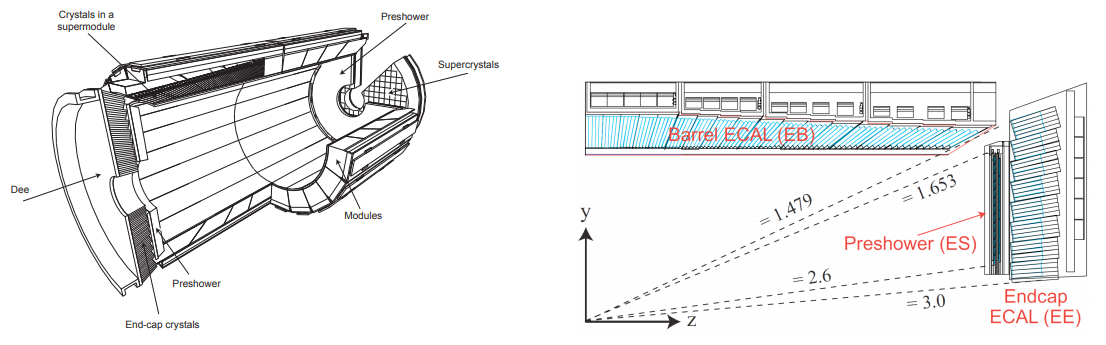
\includegraphics[width=7in]{Chapter3/importfigs/ecal_performance_with_examples.png}
\par\end{centering}
\caption{ECAL components \label{fig:ecalComp}}
\end{figure}

The data readout is fast enough that CMS can trigger off signals in the ECAL. It takes about 25 ns for an ECAL hit to scintillate 80 percent of its lights, putting the calorimeter's rate on the same scale as the bunch crossing. Scintillation in the crystals activates photodetectors that transmit information to the L1 trigger. In the barrel these photodectors are avalanche photodiodes (APDs). The endcaps use vacuum phototriodes (VPTs). ECAL's energy resolution, as a function of energy, is given by fig.\ref{fig:ecalRes}. The resolution increases with energy because, at large energies, parton showers become more similar as their random fluctuations average-out.

\begin{figure}[h!]
\begin{centering}
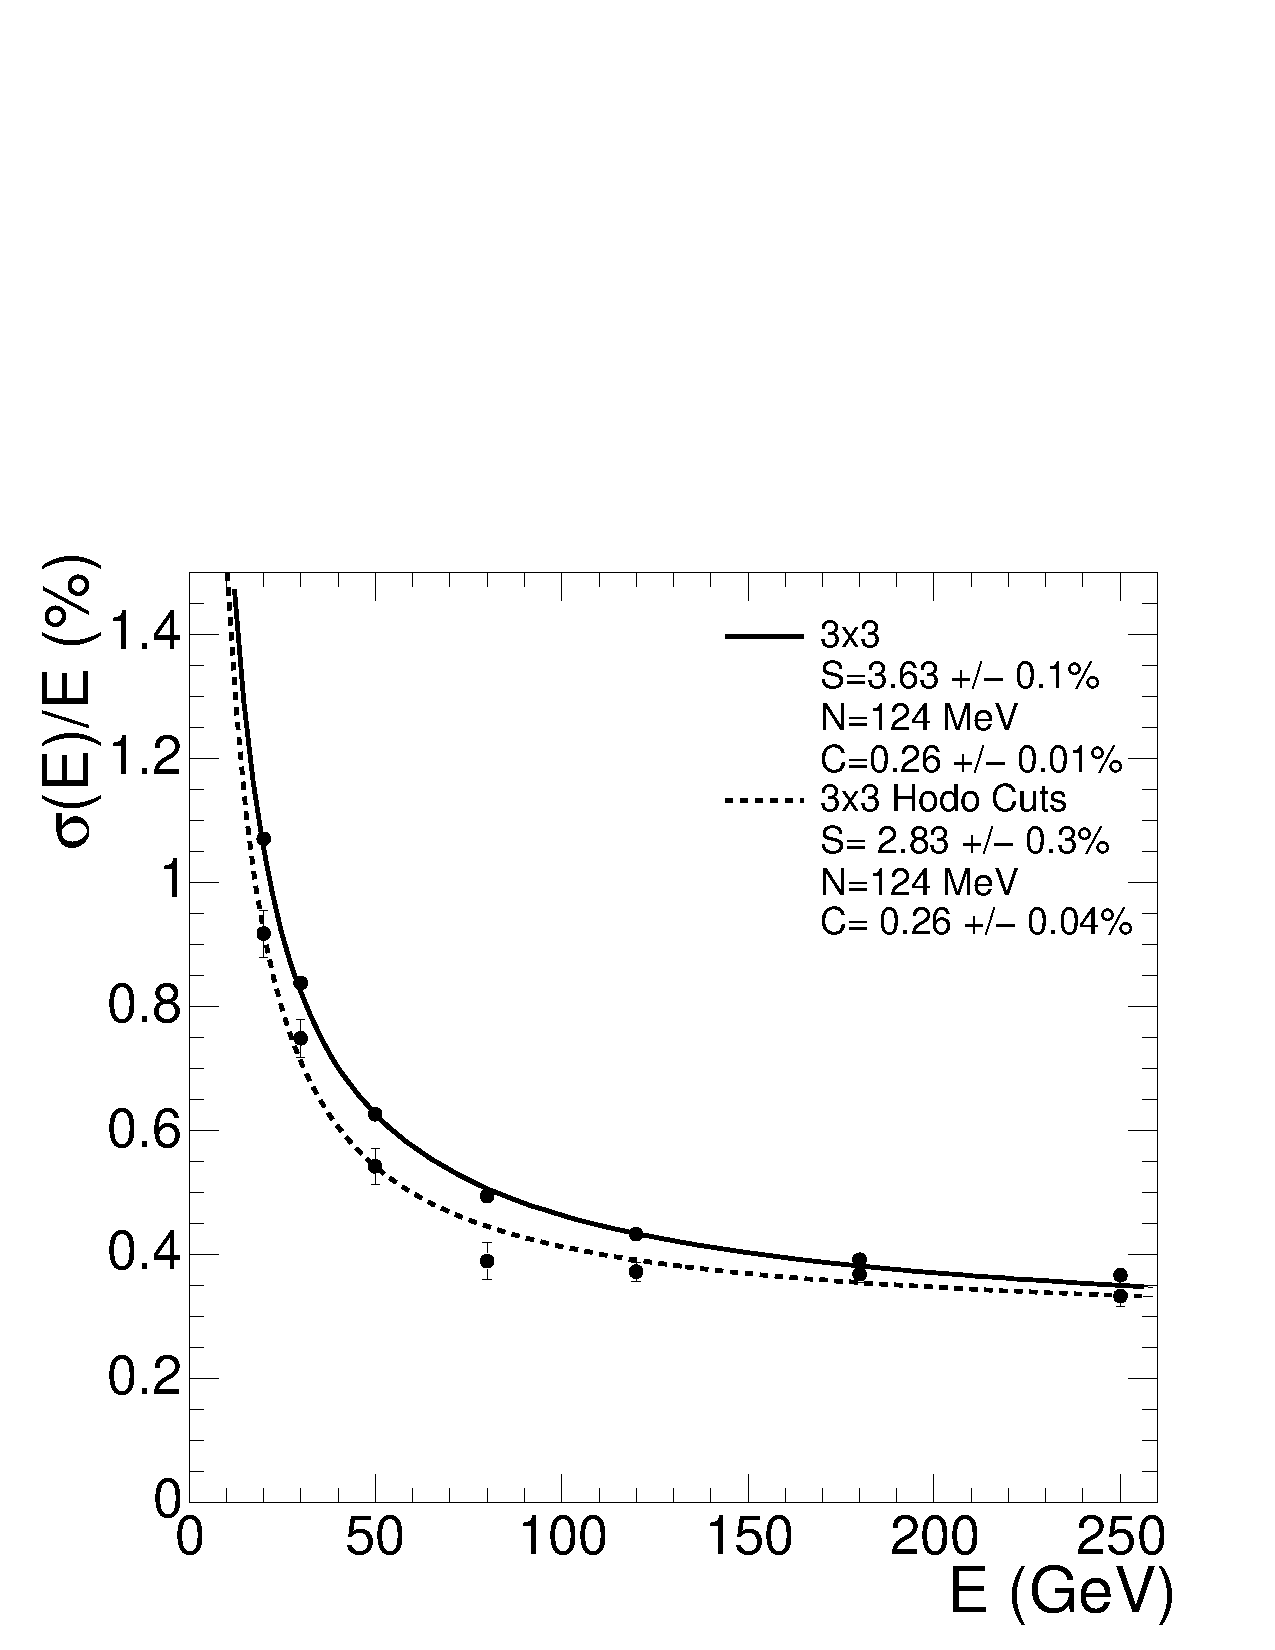
\includegraphics[width=4in]{Chapter3/importfigs/Figure_001-007.pdf}
\par\end{centering}
\caption{Ecal energy resolution \label{fig:ecalRes}}
\end{figure}
 
In CMS trigger development, "EG" triggers fire based on energy deposits in the ECAL; fig.\ref{fig:ecalResL1} gives the EG trigger energy resolution. This energy comes primarily from electrons and photons. When these particles strike a tungstate crystal, the particle shower size is approximately that of the crystal. Electrons are distinguished from photons by the correlation of track to ECAL energy. The L1 trigger does not fire on tracks, which are reconstructed at the HLT level. Thus, L1 EG triggers do not distinguish between electrons and photons. 

\begin{figure}[h!]
\begin{centering}
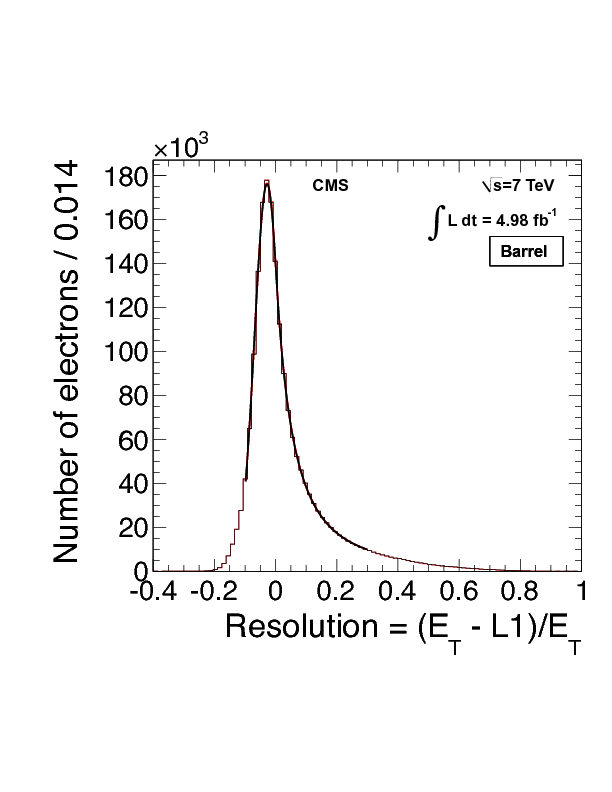
\includegraphics[width=4in]{Chapter3/importfigs/figures_L1EGresolutionEB_cmsTriggerSys.png}
\par\end{centering}
\caption{Ecal energy resolution \label{fig:ecalResL1}}
\end{figure}
 
 
\subsection{Hadronic calorimeter}


The Hadronic Calorimeter (HCAL) is the next layer outside the ECAL. The HCAL is a sampling calorimeter, meaning that it absorbs particles and measures their energyy and momentum via scintillation. HCAL has such a large acceptance that it can indirectly observe non-interacting particles such as neutrinos. The HCAL is designed to be hermetic, so that imbalances of momentum and energy can be precisely measured. Fig.\ref{fig:hcalRes} plots the HCAL's energy resolution; note that the resolution changes with $|\eta|$.

\begin{figure}[h!]
\begin{centering}
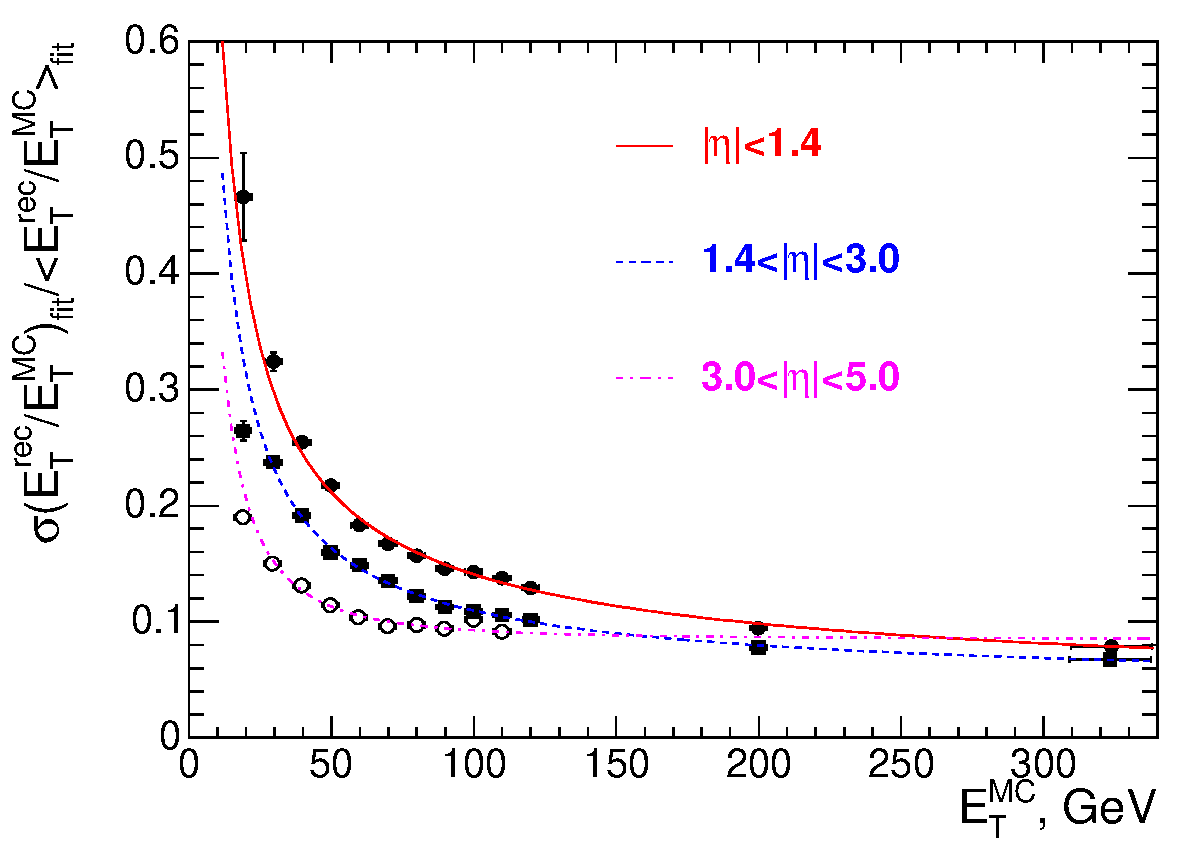
\includegraphics[width=4in]{Chapter3/importfigs/Figure_001-008.pdf}
\par\end{centering}
\caption{HCAL energy resolution \label{fig:hcalRes}}
\end{figure}

There are four sub-sections of the HCAL: the inner barrel (HB) and the outer barrel (HO), two endcaps (HE), and two forward calorimeters (HF). The HF are the most relevant to this analysis because of their use in triggering on non-hadronic events. Fig.\ref{fig:hcalComp} shows the HCAL energy resolution.

\begin{figure}[h!]
\begin{centering}
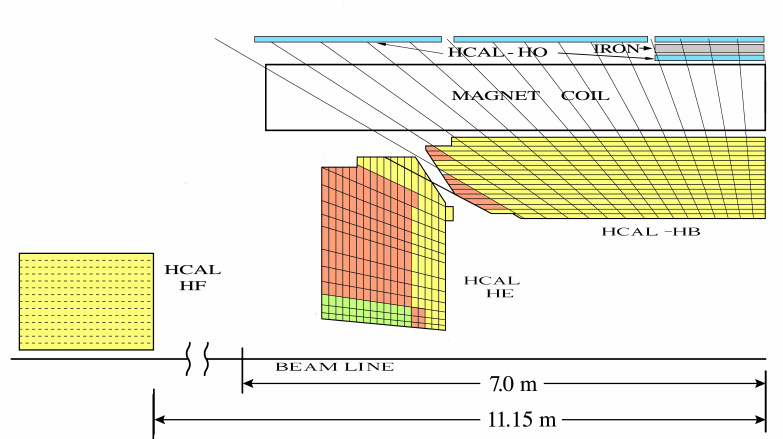
\includegraphics[width=5in]{Chapter3/importfigs/filtering_noise_in_CMS_hadron_calorimeter.png}
\par\end{centering}
\caption{HCAL Components \label{fig:hcalComp}}
\end{figure}


\subsubsection{Hadronic forward calorimeters}

The Hadronic Forward Calorimeters (HF) absorbs the greatest portion of energy from collisions. As named, it is located in the forward region ($3.0<|\eta| < 5.2 $) of CMS and complements the coverage provided by the barrel and endcap detectors.

HCAL is of made of quartz fibers and steel absorbers for maximum radiative resistance. When high energy particles pass through the quartz fibers, these particles are moving faster than the speed of light in the medium, depositing energy that causes particle showers. These showers give off light, in the form of Cherenkov radiation, that the fibers transmit to photomultiplier tubes (PMTs). The PMTs readout to the L1-trigger. Triggering on HF can also be done by vetoing on HF activity.

Hits in the HF are used to measure the instantaneous luminosity of CMS. As shown in fig.\ref{fig:hcalRes}, the HF have a finer $E_T$ resolution than the other parts of the HCAL, making it suitable for high precision measurement of luminosity. Furthermore, because HF noise is comparatively small with respect to Minbias HF threshold, the veto of the HF threshold is a reliable measure of HF "emptiness". 

\subsection{Muon detector}

The outermost layer of CMS consists of the muon detectors, as seen in fig.\ref{fig:muonYZ}. Muons are particles nearly identical to electrons, except for their mass, which exceeds that of the electron by some two orders of magnitude. High mass particles, like the Higgs boson, often decay into a final state containing muons. The muon detector not only identifies muons, but also measures their momentum. The muon detector has readout fast enough for triggering on muons.

\begin{figure}[h!]
\begin{centering}
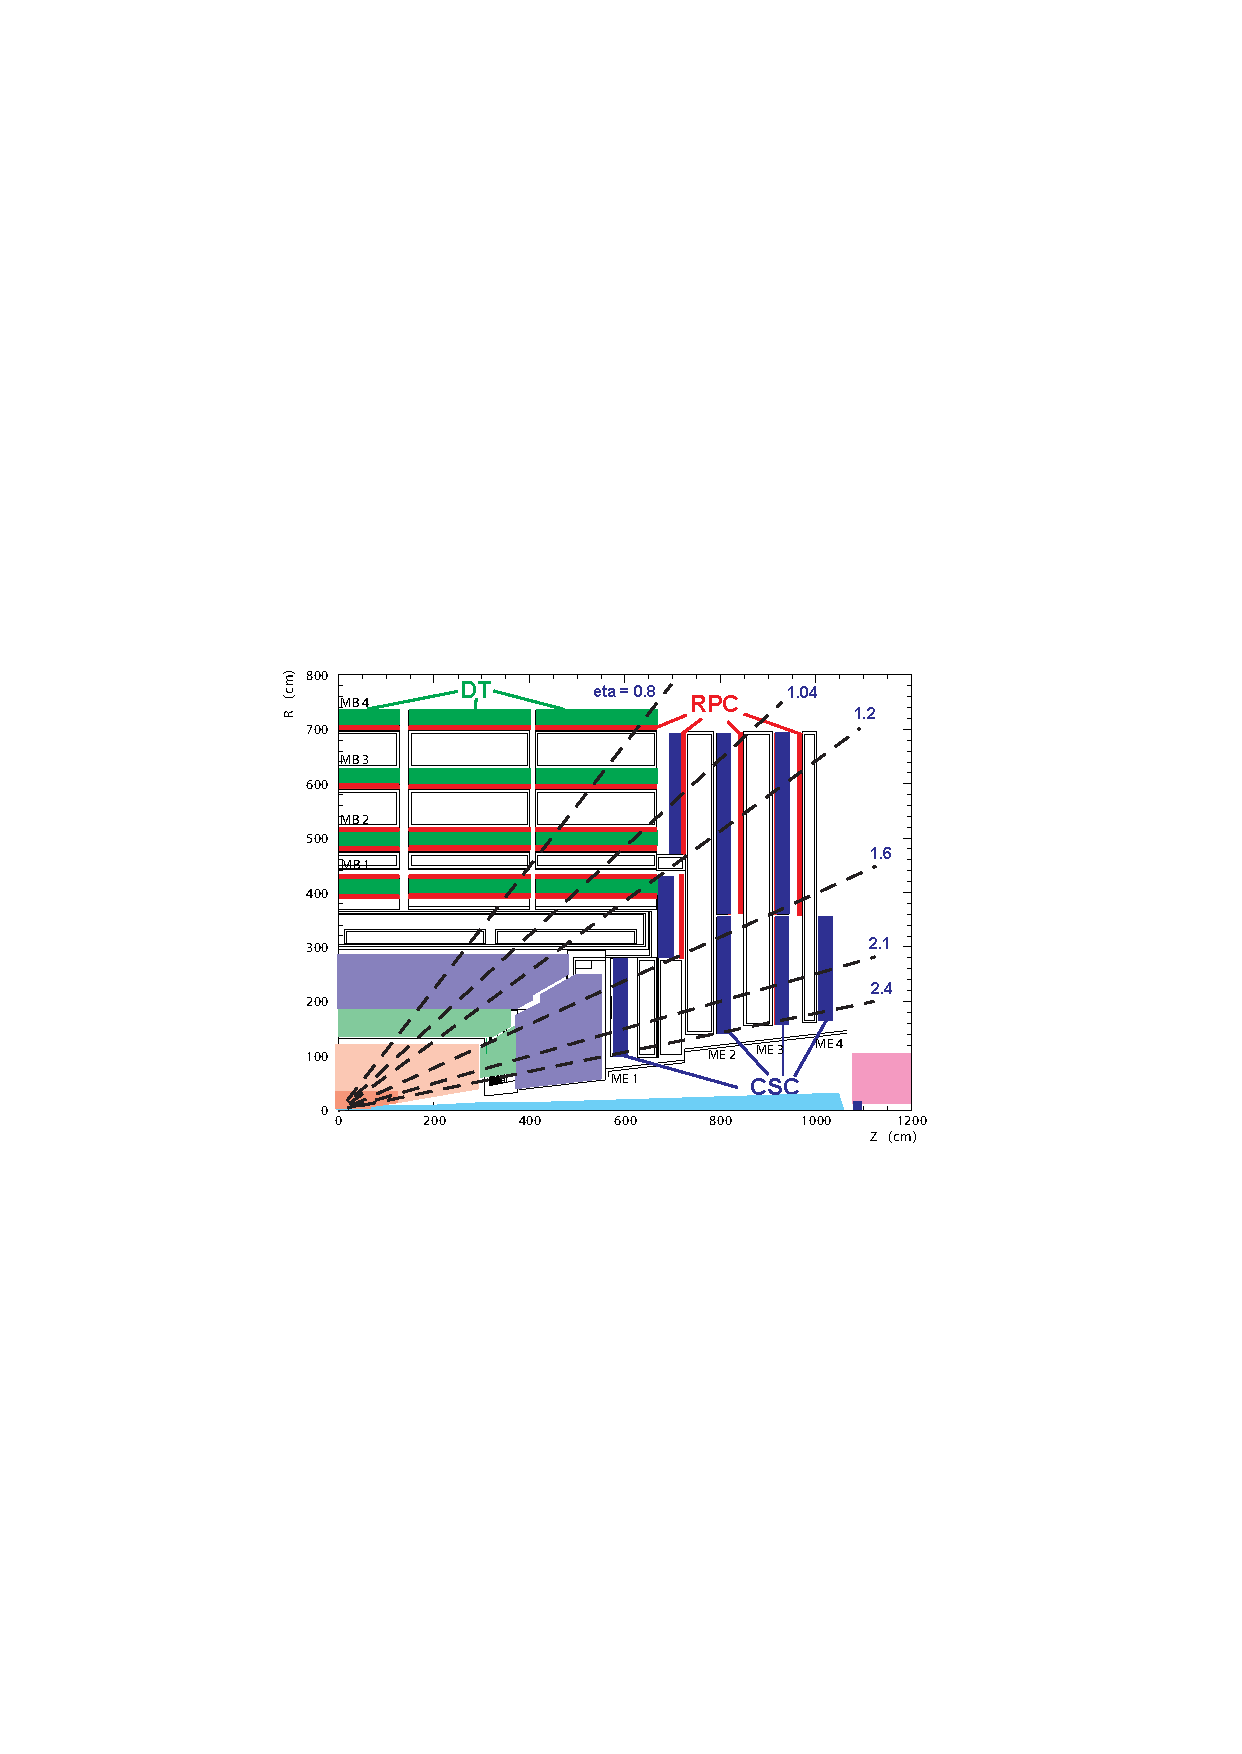
\includegraphics[width=4in]{Chapter3/importfigs/Figure_001-006.pdf}
\par\end{centering}
\caption{Pseudorapidity acceptance of muon detector \label{fig:muonYZ}}
\end{figure}

The muon detector consists of three types of component: muon drift tubes (DT), cathode strip chambers (CSC), and resistive plate chambers (RPC). The DTs are gas filled chambers that contain a stretched metal wire. When muons pass through the DT gas, electrons are excited. These electrons escape from the gas atoms and are attracted to the metal wire, which triggers a signal. The CSC, located in the endcaps, operate under similar principles, but contain perpendicular arrays of positively charged and negatively charged wires immersed in gas. The RPC do not use electrode wires to detect excited electrons; instead, high-resitivity plates are used as alternating cathodes and anodes. 

\subsection{Zero degree calorimeter}

The zero degree calorimeters are both sides of CMS, approximately 140 meters from the interaction point. Each ZDC consists of two independent systems: an electromagnetic calorimeter, for detecting very forward photons, and a hadronic calorimeter, for detecting neutrons. Because these neutrons result from the dissociation of nuclei, the ZDC can measure the centrality of heavy-ion collisions. Hadrons in the forward region have energy on the TeV scale, so the ZDC's hadronic calorimeter is made of thick tungsten plates. For a UPC process, the photon emitting nucleus is most likely to remain intact; therefore, ZDC data can the photon direction of a process, and by extension it's energy. 

\subsection{Particle flow algorithm}

Raw data from the sub-detectors is combined, for data analysis, by the particle-flow (PF) algorithm. The PF takes the data about tracks in the tracker and energy deposits in the calorimeter, and uses them to reconstruct physics-related data objects, like jets, and to identify specific particles, such as photons and muons. The PF also identifies missing energy and momentum for use in neutrino studies. These data objects are stored in a format similar to that of conventional MC event generators. CMS gains significant jet reconstruction efficiency via the PF. At low transverse momentum, PF reconstructs jets at nearly twice the resolution of HCAL and ECAL. This increase in efficiency comes from the PF integrating in track data with the calorimeter tower data. Fig.\ref{fig:pfPerf} compares the performance of the PF algorithm to the calorimter reconstruction.

\begin{figure}[h!]
\begin{centering}
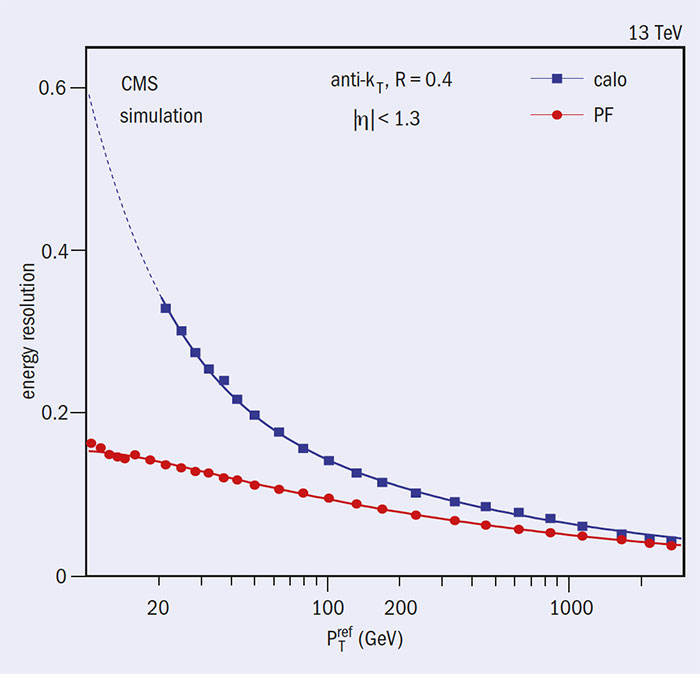
\includegraphics[width=4in]{Chapter3/importfigs/CCrec2_05_16.jpg}
\par\end{centering}
\caption{Performance of particle flow alorgithm compared to calorimeter readout.\label{fig:pfPerf}}
\end{figure}


